\documentclass[11pt,a4paper]{article}
\usepackage{fontspec}
\usepackage{polyglossia}
\setmainlanguage{russian}
\setotherlanguage{english}
\IfFontExistsTF{Times New Roman}{\setmainfont{Times New Roman}}{\setmainfont{Libertinus Serif}}
\IfFontExistsTF{Menlo}{\newfontfamily\cyrillicfonttt{Menlo}}{\newfontfamily\cyrillicfonttt{DejaVu Sans Mono}}
\usepackage[a4paper,top=2cm,bottom=2cm,left=2.1cm,right=2.1cm]{geometry}
\usepackage{graphicx}
\usepackage{booktabs}
\usepackage{tabularx}
\usepackage{array}
\usepackage{float}
\usepackage{caption}
\usepackage{enumitem}
\usepackage{amsmath,amssymb}
\usepackage{xurl}
\usepackage{hyperref}
\hypersetup{colorlinks=true,linkcolor=black,citecolor=black,urlcolor=blue}
\graphicspath{{metrika_project_images/}}
\setlength{\parindent}{1.25em}
\setlength{\parskip}{0.45em}
\setlength{\emergencystretch}{3em}
\linespread{1.04}\selectfont
\captionsetup{font=small,labelfont=bf}
\setlength{\textfloatsep}{10pt plus 2pt minus 2pt}
\setlength{\intextsep}{10pt plus 2pt minus 2pt}
\setlist[itemize]{topsep=3pt,itemsep=2pt,parsep=0pt,leftmargin=1.6em}
\begin{document}

\begin{titlepage}
\centering
{\large Федеральное государственное автономное образовательное учреждение высшего образования\par}
{\large НАЦИОНАЛЬНЫЙ ИССЛЕДОВАТЕЛЬСКИЙ УНИВЕРСИТЕТ\par}
{\large «ВЫСШАЯ ШКОЛА ЭКОНОМИКИ»\par}
{\large Факультет экономических наук\par}
{\large Эконометрика\par}
\vfill
{\Large\bfseries Эмпирическая оценка влияния степени загрязнения воздуха на ожидаемую продолжительность жизни в регионах Российской Федерации\par}
\vfill
\begin{flushright}\textbf{Выполнили:}\end{flushright}
\begin{flushright}Ковалёва Мария Сергеевна\end{flushright}
\begin{flushright}Кутузов Иван Владимирович\end{flushright}
\begin{flushright}Николюк Татьяна Николаевна\end{flushright}
\begin{flushright}\textbf{Преподаватель семинаров:}\end{flushright}
\begin{flushright}Бывальцева-Станкевич Анастасия Александровна\end{flushright}
\vfill
{\large г. Москва, 2026 г.\par}
\end{titlepage}

\section*{Введение}
Загрязнение атмосферного воздуха - одна из наиболее значимых экологических и социально-экономических проблем современности. По оценкам Всемирной организации здравоохранения, загрязнение воздуха связано с повышенным риском сердечно-сосудистых, респираторных и онкологических заболеваний, что непосредственно негативно влияет на качество и ожидаемую продолжительность жизни. Для России данная проблема вызывает особый интерес вследствие высокой неоднородности регионов по уровню промышленной нагрузки, энергетической структуры экономики и концентрации вредных выбросов. В ряде субъектов РФ сохраняется высокий уровень загрязнения атмосферы, связанный с деятельностью металлургии, теплоэнергетики, добывающей промышленности и тяжелого производства.

Таким образом, становится важным в рамках данного исследования определить влияние загрязнения воздуха на ожидаемую продолжительность жизни в регионах РФ для возможной корректировки политики в сторону улучшения экологической обстановки, а также повышения осведомленности населения об угрозе для жизни в их регионе, представленной высокой концентрацией токсичных веществ в атмосферном воздухе.

\section*{Цель исследования}
Цель данного эмпирического исследования - оценка статистической значимости, силы и направления влияния степени загрязнения воздуха на ожидаемую продолжительность жизни населения по субъектам РФ.

Дополнительно исследование направлено на:

\begin{itemize}
\item выявление факторов, которые являются причиной региональных различий в продолжительности жизни;
\item проверку наличия эндогенности между загрязнением и иными характеристиками регионов;
\item оценку применимости инструментальных переменных для идентификации и борьбы с эндогенностью.
\end{itemize}
\section*{Актуальность исследования}
Высокий риск смертности, связанный с сильным загрязнением воздуха, остается актуальной проблемой во всем мире. Это подтверждается ежегодными отчетами “State of Global Air” от исследовательских организаций Health Effects Institute и Institute for Health Metrics and Evaluation. Так, например, в отчете на 2025 г. подчеркивается, что загрязнение воздуха остается вторым ведущим риск-фактором ранней смерти, уступая только высокому кровяному давлению.

Кроме того, в 2023 году во всем мире 7.9 млн смертей были связаны с загрязнением атмосферы, которая включает в себя концентрацией PM2.5 (микрочастиц), загрязнение воздуха домашних хозяйств и воздействие озона, содержание которого сейчас на 30-70\% выше, чем 100 лет назад. В глобальном распределении смертности, связанной с загрязнением воздуха, центральная и восточная Европа вместе с центральной Азией занимают 4.5\%, что невелико в сравнении с югом и востоком Азии и Океанией (в совокупности 68.2\%), но по-прежнему значимо в рамках региональной проблемы.

Важность проблемы мирового загрязнения воздуха подчеркивается также и в отчете Института энергетической политики Чикагского университета “Air Quality Life Index Annual Update” 2025 г., в котором отмечается, что в 2023 г. глобальная концентрация PM2.5 повысилась на 1.5\% в сравнении с 2022 г. и почти в 5 раз превысила рекомендуемый ВОЗ уровень в 5 µg/m³, достижение которого обеспечила бы повышение средней продолжительности жизни примерно на 1.9 лет, что в общей сложности увеличило бы численность населения планеты на 15.1 млрд лет. Таким образом, отчет напрямую интерпретирует загрязнение воздуха через потери ожидаемой продолжительности жизни, что соответствует логике настоящего исследования. Также он повествует и о положительных изменениях в экологической политике стран, направленной на снижение атмосферного загрязнения, например, о введении Евросоюзом в 2024 г. ограничения на концентрацию PM2.5 в 10 µg/m³ до конца 2030 г., что безусловно влияет на увеличение средней продолжительности жизни.

Связь смертности и загрязнения воздуха в России была описана уже более 25 лет назад в работе Б. Ревича, А. Быкова 1998 г., в которой констатировалась 7\% смертность от загрязнения воздуха только взвешенными веществами для населения в 15 млн. Кроме того, авторы призывают к детальному рассмотрению этой темы и новым исследованиям.

Немаловажной в рамках темы является статья V.P. Reshetin, V.I. Kazazyan “Public-Health Impact of Outdoor Air Pollution in Russia” 2004 г., основой которой послужили данные мониторинга Росгидромета за 1993 и 1998 годы. По их расчетам, загрязнение воздуха частицами может быть связано с 219-233 тыс. преждевременных смертей или 15-17\% смертности в год.

Авторы подчеркивают необходимость внедрения мер по снижению экологических рисков в городах РФ.

С 2018 г. в стране действует национальный проект «Чистый воздух», направленный на снижение выбросов в 12 наиболее загрязненных городах. Но несмотря на всю практическую значимость проблемы, эконометрическая литература по причинному эффекту загрязнения на продолжительность жизни на российских данных остается крайне ограниченной, что подчеркивает необходимость проведения исследования.

\section*{Гипотезы исследования}
\paragraph{Гипотеза 1: Рост выбросов загрязняющих веществ на душу населения сокращает ожидаемую продолжительность жизни в регионах РФ}
\begin{center}\small H$_0$: β$_1$ = 0 (выбросы не влияют на ОПЖ) \\ H$_1$: β$_1$ < 0 (рост выбросов сокращает ОПЖ)\end{center}
Ожидаемое направление: β$_1$ < 0 в спецификации (3).

В обоснование гипотезы можно привести несколько работ. Pope et al. (2002) показали на данных American Cancer Society, что рост долгосрочной концентрации PM$_2$.$_5$ на 10 мкг/м³ увеличивает сердечно-сосудистую и легочную смертность примерно на 6\% и 8\%. Chen et al. (2013) и Ebenstein et al. (2017) на данных о реке Хуайхэ оценили потери продолжительности жизни на севере Китая (с большей концентрацией выбросов) в 3-5 лет. Currie \& Neidell (2005) добавляют, что значимые эффекты на здоровье фиксируются даже при относительно невысоких уровнях экспозиции (низких уровнях загрязнения воздуха). Наконец, Ревич и Быков (1998) оценили избыточную смертность от атмосферных выбросов непосредственно для крупных городов России.

\paragraph{Гипотеза 2: После контроля на загрязнение воздуха и базовые социально-экономические характеристики более высокий доход на душу населения положительно связан с ОПЖ}
\begin{center}\small H$_0$: β\_grp\_pc = 0 (доход не связан с ОПЖ при прочих равных) \\ H$_1$: β\_grp\_pc > 0 (более богатые регионы живут дольше при фиксированном уровне загрязнения)\end{center}
Preston (1975) показал устойчивую положительную связь между национальным доходом на душу населения и ОПЖ в межстрановом разрезе, однако подчеркнул, что значительная часть вариации определяется факторами, экзогенными доходу. В российских регионах сырая корреляция отрицательна (r = -0,13), что отражает специфику сырьевых территорий: высокий ВРП здесь сопряжен с промышленной нагрузкой, суровым климатом и специфической структурой занятости, а не с теми механизмами улучшения здоровья, которые описывает Preston. Соответственно, мы ожидаем, что β̂\_grp\_pc > 0.

\paragraph{Гипотеза 3. Занятость в добыче полезных ископаемых на душу населения связана с уровнем загрязнения воздуха после учёта контрольных переменных}
\begin{center}\small H$_0$: π\_1 = 0 \\ H$_1$: π\_1 > 0\end{center}
Проверка релевантности - необходимое условие 2SLS. Добыча - отрасль с высокой эмиссионной интенсивностью на занятого (в связи с чем ожидаем π\_1 > 0). Greenstone (2002) и Chay \& Greenstone (2003) показали, что отраслевая структура региона по американским данным - один из главных экзогенных факторов локального уровня загрязнения.

\section*{Данные}
В работе были использованы кросс-секционные данные по 85 регионам России за 2015 год, так как именно за этот год данные имелись в наиболее полном объеме. Основной источник данных- Fedstat, ссылки на конкретные датасеты представлены в приложении. Все переменные, описанные ниже, являются непрерывными количественными. Еще используется переменная region- категориальная. В моделях также используются логарифмы некоторых переменных.

\subsection*{Зависимая переменная}
\begin{center}\small life\_expectancy- ожидаемая продолжительность жизни в годах, основной показатель здоровья населения\end{center}
\subsection*{Основная объясняющая переменная}
emissions\_h1\_pc- выбросы загрязняющих веществ от стационарных источников на душу населения, тыс. тонн на человека

\subsection*{Инструментальные переменные}
\begin{itemize}
\item emp\_mining\_pc- занятость в добыче полезных ископаемых на душу населения, основной инструмент;
\item emissions\_fuel\_pc- выбросы от сжигания топлива на душу населения;
\item emp\_energy\_pc- занятость в энергетике на душу населения.
\end{itemize}

\subsection*{Контрольные переменные}
\begin{itemize}
\item grp\_pc- ВРП на душу населения, тыс. руб. на человека;
\item urban\_share- доля городского населения;
\item age\_struct\_share- доля населения старших возрастов (используется прежде всего как robustness-переменная);
\item population\_avg- среднегодовая численность населения, человек.
\end{itemize}

\subsection*{Дополнительные переменные}
\begin{itemize}
\item industrial\_index- индекс промышленного производства;
\item visits\_per\_capita- число посещений лечебных учреждений на одного жителя;
\item emp\_manufacturing\_pc- занятость в обрабатывающих производствах на душу населения;
\item emp\_construction\_pc- занятость в строительстве на душу населения;
\item emp\_metallurgy\_pc- занятость в металлургии на душу населения;
\item emp\_chemicals\_pc- занятость в химическом производстве на душу населения.
\end{itemize}

\section*{Методы и спецификация модели}
Оценивание проводится в два шага. Сначала строится базовая OLS-регрессия - она дает состоятельные оценки только при отсутствии эндогенности, которая здесь может присутствовать. Затем применяется 2SLS, где в качестве инструмента для эндогенной переменной ln\_emissions\_h1\_pc выступает логарифм занятости в добыче полезных ископаемых на душу населения. Во всех спецификациях стандартные ошибки скорректированы на гетероскедастичность (HC1).

Базовая OLS-регрессия (уравнение 1):

\begin{center}\small life\_expectancy\_i = β\_0 + β\_1 * ln\_emissions\_h1\_pci + β\_2 * ln\_grp\_pc\_i + β\_3 * urban\_share\_i + β\_4 * ln\_population\_avg\_i + ε\_i\end{center}
Первая ступень 2SLS (уравнение 2):

\begin{center}\small ln\_emissions\_h1\_pc\_i = π\_0 + π\_1 * ln\_emp\_mining\_pc\_i + π\_2 * ln\_grp\_pc\_i+π\_3 * urban\_share\_i + π\_4* ln\_population\_avg\_i + v\_i\end{center}
Вторая ступень 2SLS (уравнение 3):

\begin{center}\small life\_expectancy\_i = β\_0 + β\_1 * fitted\_ln\_emissions\_h1\_pc\_i + β\_2 * ln\_grp\_pc\_i + β\_3 * urban\_share\_i + β\_4 * ln\_population\_avg\_i + ε\_i\end{center}
Логарифмическая форма для выбросов, ВРП и численности населения выбрана из-за правосторонней асимметрии этих переменных. Коэффициент β$_1$ интерпретируется как полу-эластичность: изменение ОПЖ в годах при удвоении выбросов на душу населения равно β$_1$ · ln 2 ≈ β$_1$ · 0,693.

Инструмент ln\_emp\_mining\_pc выбран как основной, потому что занятость в добыче определяется прежде всего геологическим размещением ресурсов и отраслевой структурой региона, а добывающие отрасли являются одним из крупнейших источников стационарных выбросов. При этом условие исключения не может быть проверено напрямую и не является механически гарантированным. Добывающие регионы могут отличаться не только уровнем загрязнения, но и климатом, инфраструктурой, структурой занятости, доходами, миграционными потоками.

\section*{Эндогенность и инструментальная стратегия}
OLS-оценка β$_1$ из уравнения (1) смещена как минимум в силу:

\begin{itemize}
\item пропущенных переменных - качество здравоохранения, климат, исторически сложившаяся отраслевая структура связаны одновременно и с загрязнением, и с продолжительностью жизни;
\item ошибок измерения в emissions\_h1, которая не учитывает транспорт, бытовое отопление и трансграничный перенос;
\item миграционных причин - здоровые трудоспособные граждане концентрируются в индустриальных регионах, искусственно завышая продолжительность жизни там.
\end{itemize}
Ожидается, что |β̂\_2SLS| > |β̂\_OLS|, что согласуется с направлением смещения, обсуждаемым выше.

В качестве инструмента используется логарифм занятости в добыче полезных ископаемых на душу населения. Его релевантность объясняется тем, что размещение добывающих производств определяется геологией и освоением территорий, а не текущей политикой здравоохранения, тогда как добыча и первичная переработка сырья - один из главных источников стационарных выбросов. Ожидается, что F-статистика первой ступени превысит порог Staiger \& Stock (1997) F > 10; в случае умеренной силы инструмента будут применены робастные к слабым инструментам методы.

\section*{Диагностика и робастность}
Планируются следующие диагностические проверки:
\begin{itemize}
\item тест Wu–Hausman / Дурбина на экзогенность регрессора;
\item проверка силы инструмента по частной F-статистике с критическими значениями Stock \& Yogo (2005);
\item VIF-анализ мультиколлинеарности;
\item тест Саргана при использовании более одного инструмента;
\item переоценка без влиятельных наблюдений (Cook's distance, leverage);
\item альтернативные инструменты - занятость в энергетике.
\end{itemize}

\section*{Ограничения}
Кросс-секция за один год не позволяет контролировать ненаблюдаемую региональную гетерогенность через фиксированные эффекты - это недостаток, который лишь частично компенсирует инструментальная переменная. Данные об emissions\_h1 охватывают только стационарные источники, исключая транспорт и бытовой сектор, что занижает суммарную экспозицию.

\section*{Предварительный анализ данных}
\begin{table}[H]
\centering
\caption{Дескриптивные статистики основных переменных}
\footnotesize
\renewcommand{\arraystretch}{1.25}
\begin{tabularx}{\textwidth}{>{\raggedright\arraybackslash}X>{\centering\arraybackslash}X>{\centering\arraybackslash}X>{\centering\arraybackslash}X>{\centering\arraybackslash}X>{\centering\arraybackslash}X}
\toprule
\textbf{} & \textbf{mean} & \textbf{std} & \textbf{min} & \textbf{median} & \textbf{max} \\
\midrule
life\_expectancy & 70.5662 & 2.3977 & 63.14 & 70.39 & 78.47 \\
ln\_emissions\_h1\_pc & -10.3097 & 1.4159 & -14.5157 & -10.2621 & -6.9957 \\
ln\_emp\_mining\_pc & -5.5818 & 1.6311 & -8.7341 & -5.9033 & -1.5898 \\
ln\_grp\_pc & 5.85 & 0.6917 & 4.6834 & 5.7689 & 8.5867 \\
urban\_share & 70.2682 & 13.2684 & 29.9 & 71.4 & 100.0 \\
age\_struct\_share & 58.2165 & 2.0328 & 54.2 & 57.7 & 64.9 \\
ln\_population\_avg & 13.9713 & 0.9782 & 10.6546 & 13.9885 & 16.3233 \\
\bottomrule
\end{tabularx}
\end{table}

По дескриптивной статистике зависимой переменной life\_expectancy заметно, что среднее значение ожидаемой продолжительности жизни составляет 70.57 лет, стандартное отклонение – 2.4 года, минимум – 63.14 года, а максимум 78.47 лет. Такая межрегиональная вариативность достаточна для постановки вопроса о факторах, объясняющих различия в продолжительности жизни между субъектами РФ.

Кроме того, среднее значение ln\_emissions\_h1\_pc составляет около -10.31, стандартное отклонение – 1.42. Поскольку переменная находится в логарифмах, разница между минимумом (-14.52) и максимумом (-7) имеет мультипликативный смысл. Так, разница между ними в исходной шкале означает различие более чем в 1800 раз. Это показывает, что загрязнение распределено крайне неоднородно: отдельные индустриальные субъекты имеют намного более высокий уровень выбросов, чем регионы с низкой промышленной концентрацией.

Распределение ln\_emp\_mining\_pc также характеризуется большим размахом. Это отражает структурную неоднородность регионов РФ: добыча полезных ископаемых сконцентрирована в ограниченном числе ресурсных субъектов. С точки зрения IV-стратегии это означает, что первая ступень и итоговые 2SLS-оценки могут быть чувствительны к отдельным ресурсным регионам, поэтому необходима проверка устойчивости без влиятельных наблюдений.

\begin{figure}[H]
\centering
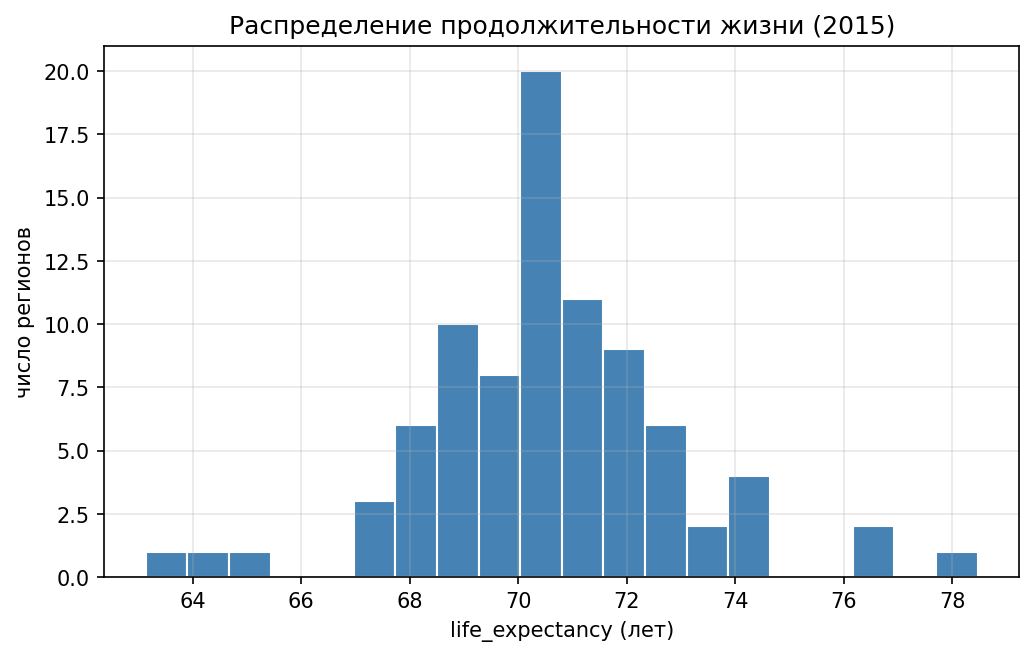
\includegraphics[width=0.82\textwidth]{image_1.png}
\caption{Распределение ожидаемой продолжительности жизни по регионам РФ}
\end{figure}

\begin{figure}[H]
\centering
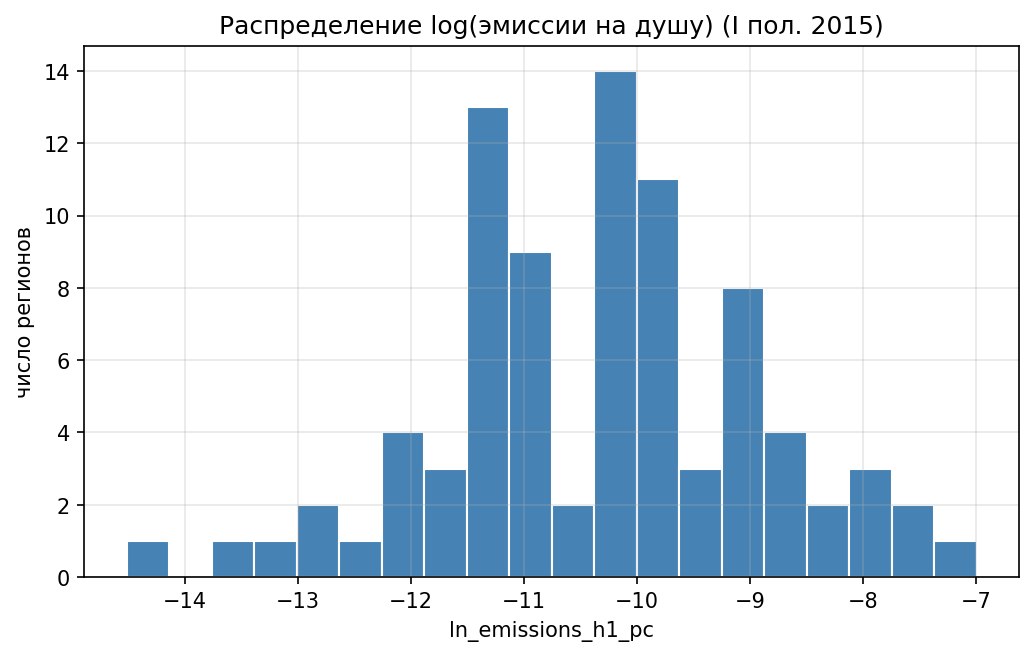
\includegraphics[width=0.82\textwidth]{image_2.png}
\caption{Распределение логарифма выбросов загрязняющих веществ на душу населения}
\end{figure}

\begin{figure}[H]
\centering
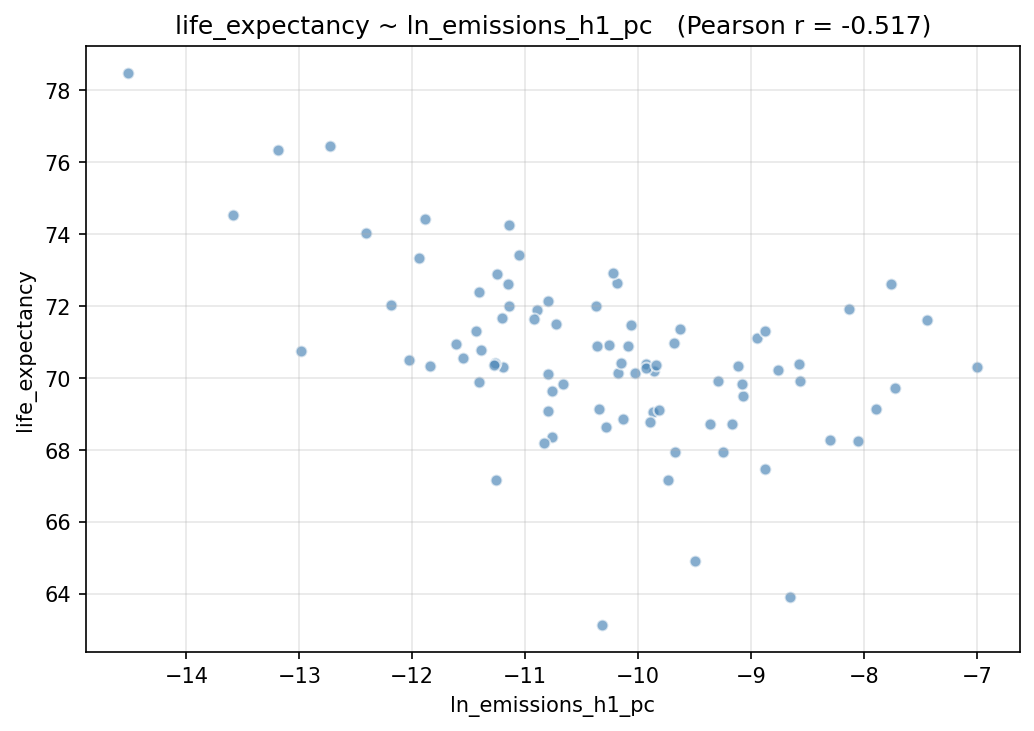
\includegraphics[width=0.82\textwidth]{image_3.png}
\caption{Связь между загрязнением воздуха и ожидаемой продолжительностью жизни}
\end{figure}

\begin{figure}[H]
\centering
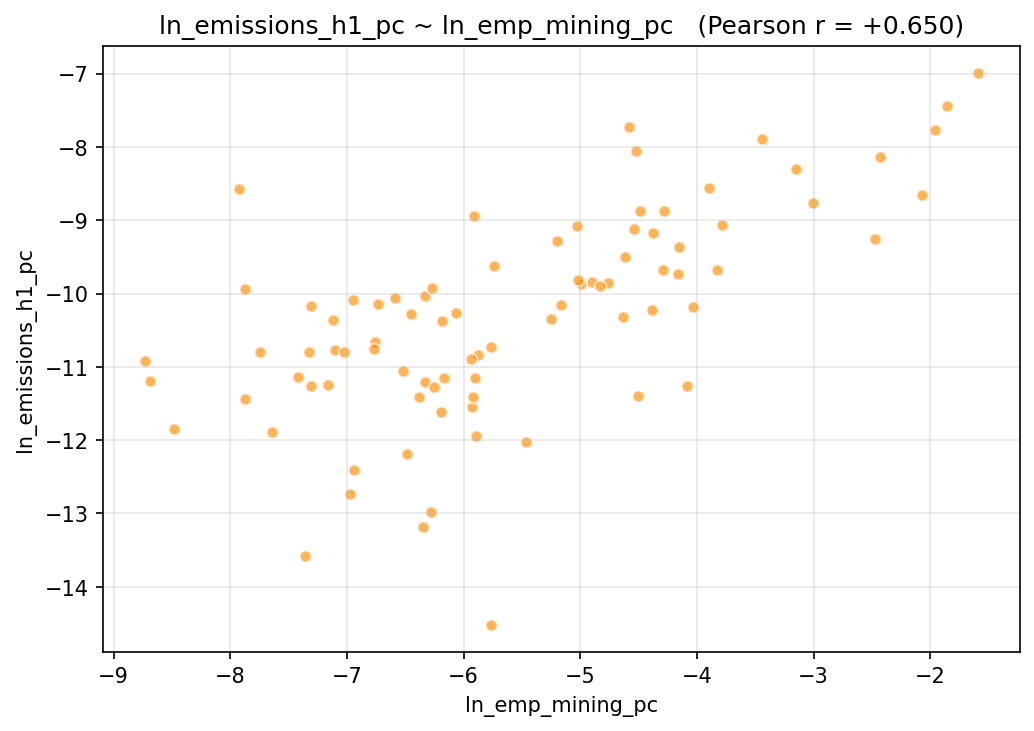
\includegraphics[width=0.82\textwidth]{image_4.png}
\caption{Связь между занятостью в добыче полезных ископаемых и загрязнением воздуха}
\end{figure}

\begin{figure}[H]
\centering
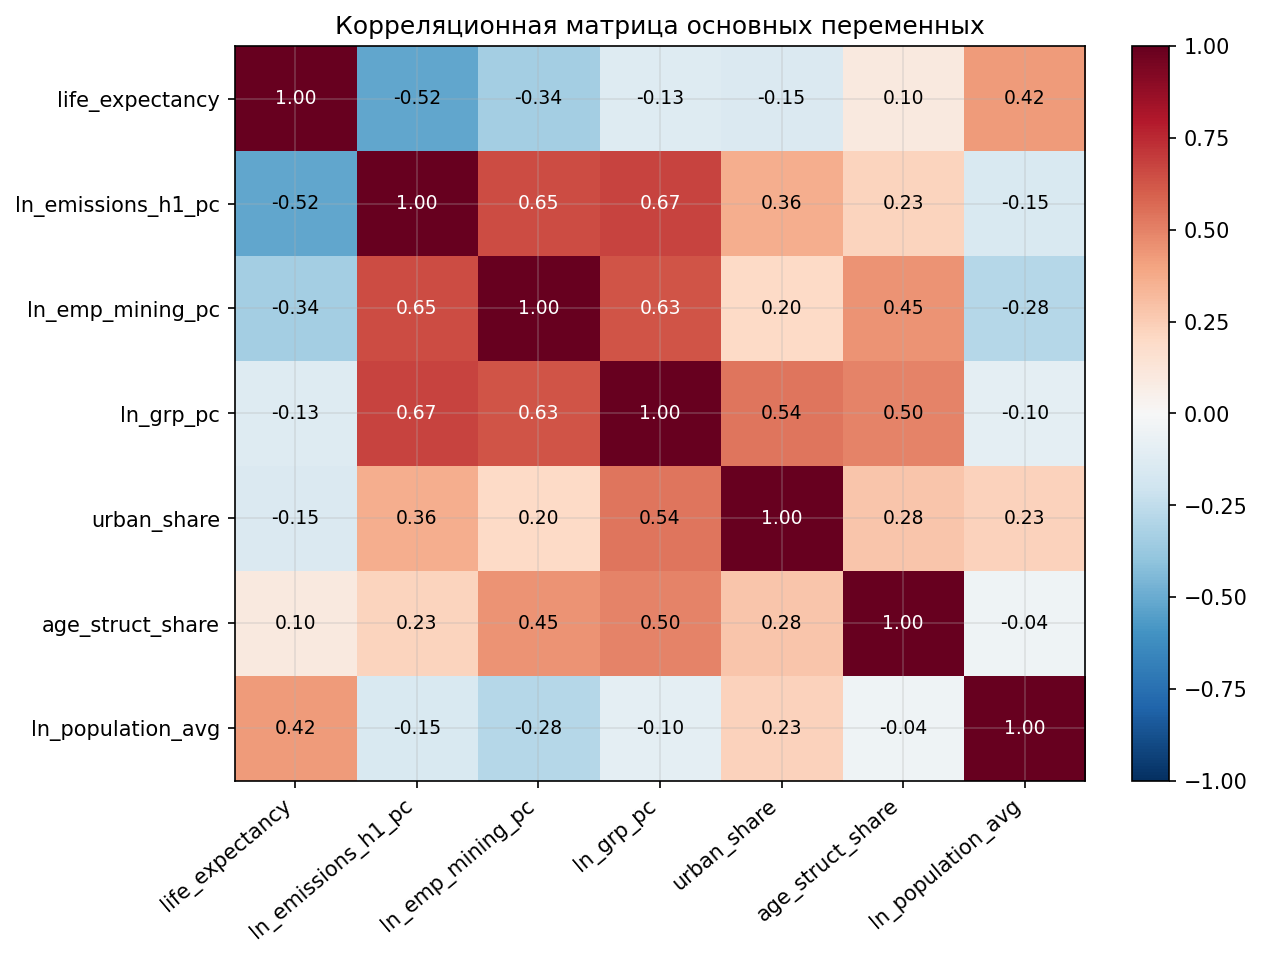
\includegraphics[width=0.82\textwidth]{image_5.png}
\caption{Корреляционная матрица основных переменных}
\end{figure}

Предварительный анализ данных позволил сделать несколько содержательных выводов:

\begin{itemize}
\item По некоторым показателям, таким как загрязнение воздуха, значения будут существенно различаться, что объясняется тем, что в регионах разный уровень развития промышленности.
\item Распределение выбросов заметно асимметрично, так что данная переменная обоснованно прологарифмирована.
\item Между ОПЖ и загрязнением воздуха наблюдается умеренная отрицательная корреляция (-0.52), что согласуется с основной гипотезой исследования.
\item Занятость в добыче положительно связана с загрязнением (0.65), что подтверждает релевантность инструмента.
\item Некоторые корреляции также указывают на потенциальную проблему смешения эффектов: загрязнение, ВРП, добывающая занятость и урбанизация связаны между собой. Следовательно, отрицательная связь между загрязнением и ОПЖ может частично отражать не только экологический эффект, но и степень индустриализации регионов.
\item Именно поэтому далее необходимы множественная регрессия, контроль социально-экономических факторов и IV-подход.
\end{itemize}
\section*{Данные и изменения после proposal}
В финальной версии были внесены три важных уточнения относительно proposal.

\begin{itemize}
\item \textbf{Проверка автономных округов.} В финальной версии датасета используется исправленная версия, где Архангельская область и Тюменская область берутся без автономных округов, чтобы избежать эффекта двойного подсчета.
\item \textbf{Возрастная структура.} age\_struct\_share не включается в основную модель, поскольку демографическая структура может частично определяться самим исследуемым результатом: высокая или низкая доля отдельных возрастных групп может отражать прошлую смертность, миграцию и региональную селекцию. Поэтому она используется только в проверках робастности.
\item \textbf{Обращаемость в медучреждения.} visits\_per\_capita не включается в основную модель. Эта переменная может отражать не только доступность медицины, но и текущую заболеваемость, то есть сама быть связанной с результатом.
\end{itemize}

Переменная region используется только как идентификатор наблюдений и не включается в модели как категориальный регрессор.

\section*{Дополнительное описание переменных}
\begin{itemize}
\item Ключевая объясняющая переменная emissions\_h1\_pc, то есть выбросы загрязняющих веществ от стационарных источников на душу населения. В основной спецификации используется ее логарифм ln\_emissions\_h1\_pc, что обосновано статистически и содержательно. Статистически эта переменная имеет выраженную правостороннюю асимметрию: большинство регионов характеризуется относительно умеренными выбросами, тогда как отдельные ресурсные и индустриальные регионы имеют экстремально высокие значения.
\item Переменная ln\_grp\_pc отражает логарифм ВРП на душу населения и используется как контроль уровня экономического развития региона. Более высокий ВРП на душу населения может быть связан с лучшей инфраструктурой, большей доступностью медицинских услуг и, следовательно, с более высокой ожидаемой продолжительностью жизни. Однако в российской региональной выборке этот показатель неоднозначен. Высокий ВРП на душу населения часто характерен для сырьевых регионов, где выше промышленная нагрузка.
\item Переменная urban\_share отражает долю городского населения, включена как контроль различий в типе расселения и уровне урбанизации, но ее ожидаемый знак неоднозначен. С одной стороны, городские регионы имеют лучшую доступность медицинской помощи и более развитую инфраструктуру, что может положительно влиять на ожидаемую продолжительность жизни. С другой, урбанизация связана с плотностью населения, транспортной нагрузкой, концентрацией промышленных объектов и более высоким загрязнением.
\item ln\_population\_avg был включён как контроль размерности: регионы резко различаются по численности населения, и без контроля масштаба крупные агломерации и малонаселенные ресурсные территории могут оказывать непропорциональное влияние на оценку связи между загрязнением и ОПЖ. Однако эту переменную также нельзя считать полностью экзогенной. Более благоприятные регионы с высокой ОПЖ могут накапливать население через миграцию и агломерационный рост. В текущих данных корреляция между ln\_population\_avg и life\_expectancy положительна и составляет примерно 0.42. Это говорит о том, что более крупные регионы в среднем имеют более высокую ожидаемую продолжительность жизни. Но такая связь не обязательно является причинной. Она может отражать агломерационные преимущества Москвы и МО, Санкт-Петербурга, Краснодарского края и других крупных регионов.
\end{itemize}

\section*{Основные результаты оценки моделей}
\begin{table}[H]
\centering
\caption{Baseline OLS и 2SLS}
\normalsize
\renewcommand{\arraystretch}{1.23}
\begin{tabularx}{\textwidth}{>{\raggedright\arraybackslash}X>{\centering\arraybackslash}X>{\centering\arraybackslash}X}
\toprule
\textbf{} & \textbf{OLS} & \textbf{2SLS} \\
\midrule
ln\_emissions\_h1\_pc & -1,2065***\newline (0,2082) & -1,5840***\newline (0,4802) \\
ln\_grp\_pc & 1,8119***\newline (0,5004) & 2,2909***\newline (0,8110) \\
urban\_share & -0,0474***\newline (0,0152) & -0,0451***\newline (0,0153) \\
ln\_population\_avg & 1,0276***\newline (0,2444) & 0,9672***\newline (0,2323) \\
Constant & 36,4870***\newline (4,9334) & 30,4784***\newline (9,7992) \\
Observations & 85 & 85 \\
R² & 0,5169 & 0,4900 \\
Robust SE & HC1 & robust, debiased \\
\bottomrule
\end{tabularx}
\end{table}

Примечание: в скобках робастные стандартные ошибки. *** p < 0,01.

\begin{itemize}
\item В OLS коэффициент при загрязнении отрицателен и статистически значим: -1,2065. Это означает, что удвоение выбросов на душу населения связано примерно со снижением ОПЖ на 1,2065 · ln 2 ≈ 0,84 года.
\item В 2SLS оценка по модулю больше: -1,5840, что соответствует снижению примерно на 1,10 года при удвоении выбросов.
\item Более высокая по модулю IV-оценка согласуется с гипотезой о возможном смещении OLS в сторону нуля, однако различие между OLS и 2SLS следует интерпретировать осторожно с учётом умеренной силы инструмента и результатов тестов экзогенности.
\item В целом полученные оценки поддерживают H1 и согласуются с литературой о негативных последствиях долгосрочного воздействия загрязнения воздуха.
\item Коэффициент при ln\_grp\_pc положителен и значим в обеих baseline-спецификациях. Это поддерживает H2: при прочих равных более высокий региональный доход связан с большей ожидаемой продолжительностью жизни.
\item Отрицательный коэффициент при urban\_share может отражать специфику российских индустриальных регионов: более высокий уровень урбанизации часто совпадает с концентрацией промышленности, экологической нагрузкой и высокой плотностью населения.
\item Этот вывод относится к базовой модели без age\_struct\_share; возрастная структура проверяется отдельно как робастная проверка, поскольку может частично отражать накопленные различия в смертности и миграции между регионами.
\end{itemize}

\section*{Первая ступень и reduced form}
\begin{table}[H]
\centering
\caption{Первая ступень и reduced form}
\normalsize
\renewcommand{\arraystretch}{1.23}
\begin{tabularx}{\textwidth}{>{\raggedright\arraybackslash}X>{\centering\arraybackslash}X>{\centering\arraybackslash}X}
\toprule
\textbf{} & \textbf{Первая ступень\newline ln\_emissions\_h1\_pc} & \textbf{Reduced form\newline life\_expectancy} \\
\midrule
ln\_emp\_mining\_pc & 0,3035***\newline (0,1038) & -0,4808***\newline (0,1706) \\
ln\_grp\_pc & 0,7797** & 1,0559 \\
urban\_share & 0,0111 & -0,0626** \\
ln\_population\_avg & -0,0649 & 1,0700*** \\
Observations & 85 & 85 \\
F-statistic for instrument & 8,5414 & — \\
p-value & 0,0045 & 0,0048 \\
\bottomrule
\end{tabularx}
\end{table}

Примечание: первая ступень оценена с HC1 standard errors.

Первая ступень показывает положительную и статистически значимую связь добычи с выбросами: π̂1 = 0,3035, p = 0,0035–0,0045 в зависимости от реализации теста. Это поддерживает H3 как условие релевантности инструмента. Однако F = 8,54 находится ниже распространённого правила большого пальца F > 10 и ниже более строгих ориентиров Stock–Yogo. Поскольку используются робастные оценки, сравнение с классическими порогами Stock–Yogo следует трактовать эвристически. Поэтому инструмент корректнее описывать как слабый или пограничный.

Приведённая форма также имеет ожидаемый знак: регионы с большей занятостью в добыче имеют более низкую ОПЖ после тех же контролей (-0,4808, p = 0,0048). Это согласуется с общей IV-логикой, но не доказывает условие исключения.

\section*{Диагностические тесты}
\begin{table}[H]
\centering
\caption{Сводка диагностических тестов для уровня значимости в 5\%}
\footnotesize
\renewcommand{\arraystretch}{1.25}
\begin{tabularx}{\textwidth}{>{\raggedright\arraybackslash}X>{\centering\arraybackslash}X>{\centering\arraybackslash}X>{\centering\arraybackslash}X>{\centering\arraybackslash}X}
\toprule
\textbf{Тест} & \textbf{H0} & \textbf{Статистика} & \textbf{p-value} & \textbf{Вывод} \\
\midrule
First stage relevance & π1 = 0 & F(1,80) = 8,5414 & 0,0045 & H0 отвергается \\
Wu–Hausman & загрязнение экзогенно & F(1,79) = 0,6806 & 0,4119 & H0 не отвергается \\
Durbin & загрязнение экзогенно & χ²(1) = 0,7260 & 0,3942 & H0 не отвергается \\
Sargan & restrictions hold & χ²(1) = 0,8726 & 0,3502 & H0 не отвергается \\
\bottomrule
\end{tabularx}
\end{table}

Тесты Wu–Hausman и Durbin с инструментом на основе добычи не отвергают экзогенность ln\_emissions\_h1\_pc. Это не означает, что экзогенность доказана: при N = 85 и умеренной силе инструмента тесты могут иметь ограниченную мощность. Существуют теоретические основания ожидать эндогенность загрязнения. В этой ситуации OLS остается полезной описательной оценкой, а 2SLS — попыткой учесть потенциальное смещение.

VIF-анализ не указывает на серьезную мультиколлинеарность между регрессорами бейзлайна: для всех объясняющих переменных VIF находится примерно в диапазоне 1,18–2,18, стандартные ошибки не искажены. H0 не отвергается (p = 0,3502), но это не доказывает валидность инструментов, особенно если потенциальное нарушение исключающего правила у инструментов имеет похожую природу.

\section*{Влиятельные наблюдения и робастность}
Отдельно проверялись leverage и Cook’s distance. Оценки базовых моделей сохраняют все 85 наблюдений: регионы с высокой добычей и малыми населениями являются содержательно важной частью вариации, а не техническими ошибками. Наблюдения только помечаются в диагностике; удаление используется как проверка робастности

Наиболее влиятельным наблюдением является Ненецкий автономный округ. После исправления проблемы двойного учета AO его Cook’s distance равен 0,9614, leverage равен 0,4960. Это близко к строгому порогу Cook’s D > 1 и существенно выше правила 4/n = 0,0471. Высокое влияние объясняется малым населением и экстремальными показателями добычи и выбросов на душу населени.

\begin{table}[H]
\centering
\caption{Robustness: возрастная структура и Ненецкий АО}
\footnotesize
\renewcommand{\arraystretch}{1.25}
\begin{tabularx}{\textwidth}{>{\raggedright\arraybackslash}X>{\centering\arraybackslash}X>{\centering\arraybackslash}X>{\centering\arraybackslash}X>{\centering\arraybackslash}X>{\centering\arraybackslash}X}
\toprule
\textbf{Спецификация} & \textbf{N} & \textbf{OLS beta} & \textbf{OLS p} & \textbf{IV beta} & \textbf{IV p} \\
\midrule
Preferred baseline & 85 & -1,2065 & 0,0000 & -1,5840 & 0,0015 \\
Добавлен age\_struct\_share & 85 & -1,1735 & 0,0000 & -1,6058 & 0,0008 \\
Leave-one-out: Ненецкий АО & 84 & -1,0861 & 0,0000 & -1,4711 & 0,0026 \\
\bottomrule
\end{tabularx}
\end{table}

Добавление переменной возрастной структуры и исключение Ненецкого АО не меняют основной знак результата: оценка эффекта загрязнения остается отрицательной и статистически значимой. Однако age\_struct\_share не интерпретируется как чистый экзогенный демографический контроль. это именно проверка чувствительности.

\section*{Альтернативные инструменты}
Дополнительно были проверены ln\_emp\_energy\_pc и ln\_emissions\_fuel\_pc. Эти инструменты могут быть более релевантными статистически, но экономически слабее с точки зрения условия исключения. Выбросы от сжигания топлива механически связаны с загрязнением и могут напрямую входить в канал загрязнения. Занятость в энергетике может влиять на ОПЖ не только через загрязнение, но и через доходы, инфраструктуру, структуру городов и качество рабочих мест. Поэтому они не рассматриваются как предпочтитеьные инструменты.

\begin{table}[H]
\centering
\caption{Robustness: альтернативные инструменты}
\footnotesize
\renewcommand{\arraystretch}{1.25}
\begin{tabularx}{\textwidth}{>{\raggedright\arraybackslash}X>{\centering\arraybackslash}X>{\centering\arraybackslash}X>{\centering\arraybackslash}X>{\centering\arraybackslash}X}
\toprule
\textbf{Инструменты} & \textbf{IV beta} & \textbf{SE} & \textbf{First-stage F} & \textbf{Wu p} \\
\midrule
ln\_emp\_mining\_pc & -1,5840 & 0,4802 & 8,5414 & 0,4119 \\
ln\_emp\_energy\_pc & -2,0811 & 0,5312 & 8,5632 & 0,0091 \\
ln\_emissions\_fuel\_pc & -2,0553 & 0,3087 & 69,2192 & 0,0000 \\
Mining + energy & -1,9251 & 0,4267 & 5,2412 & 0,0128 \\
\bottomrule
\end{tabularx}
\end{table}

Альтернативные инструменты дают тот же отрицательный знак для влияния загрязнения, но не должны использоваться как главный аргумент в пользу причинной интерпретации. Особенно сильная “первая стадия” у ln\_emissions\_fuel\_pc не делает инструмент более убедительным: наоборот, его механическая близость к загрязнению делает условие исключения более сомнительным. Поэтому предпочтительным остаётся ln\_emp\_mining\_pc, а результаты с альтернативными инструментами как дополнительная проверка устойчивости знака.

\section*{Выводы по гипотезам}
\begin{table}[H]
\centering
\caption{Итоги проверки гипотез}
\normalsize
\renewcommand{\arraystretch}{1.23}
\begin{tabularx}{\textwidth}{>{\raggedright\arraybackslash}X>{\centering\arraybackslash}X>{\centering\arraybackslash}X}
\toprule
\textbf{Гипотеза} & \textbf{Проверка} & \textbf{Вывод} \\
\midrule
H1: рост выбросов связан со снижением ОПЖ & OLS beta = -1,2065; 2SLS beta = -1,5840; оба p-value < 0,01 & Поддерживается по знаку и значимости; причинная интерпретация осторожная \\
H2: доход положительно связан с ОПЖ & OLS beta for ln\_grp\_pc = 1,8119; 2SLS beta = 2,2909; оба p-value < 0,01 & Поддерживается в базовой модели; возрастная структура только для проверки робастности \\
H3: добыча связана с выбросами & π̂1 = 0,3035; F = 8,5414; p = 0,0045 & Релевантность поддерживается, но сила инструмента пограничная/умеренная \\
\bottomrule
\end{tabularx}
\end{table}

\begin{itemize}
\item Основной результат работы состоит в том, что более высокие выбросы от стационарных источников на душу населения устойчиво связаны с более низкой ожидаемой продолжительностью жизни в регионах РФ.
\item Отрицательный знак сохраняется в OLS, базовой 2SLS, спецификации с возрастной структурой и leave-one-out проверке без Ненецкого АО.
\item По масштабу, базовая 2SLS даёт оценку, согласно которой удвоение выбросов связано примерно со снижением ОПЖ на 1,1 года. Для сравнения: Chen et al. (2013) и Ebenstein et al. (2017) оценивают потери в 3-5 лет для севера Китая при значительно более высоком уровне загрязнения - в целом сопоставимо.
\item Полученные результаты согласуются с гипотезой о негативном влиянии загрязнения воздуха на здоровье населения, однако стоит учитывать, что у инструментальной стратегии есть ограничения и данные кросс-секционного типа.
\item Также на российских данных воспроизводится кривая Престона согласно второй гипотезе. Богатые регионы живут дольше при фиксированном уровне загрязнения.
\item Тем не менее результаты не следует формулировать как окончательное доказательство причинного эффекта. Инструмент ln\_emp\_mining\_pc является статистически релевантным и экономически более правдоподобным, чем альтернативные инструменты, но его сила не является бесспорно высокой. Тесты Wu–Hausman и Durbin не отвергают экзогенность загрязнения для preferred instrument, тогда как более статистически сильные альтернативные инструменты сами более сомнительны экономически. Отрицательная связь хорошо поддерживается данными.
\end{itemize}

\section*{Список используемой литературы}
\begin{itemize}
\item “Как загрязнение воздуха разрушает наше здоровье” – Всемирная организация здравоохранения \url{https://www.who.int/ru/news-room/spotlight/how-air-pollution-is-destroying-our-health}
\item State of Global Air Report 2025 г. \url{https://www.stateofglobalair.org/resources/report/state-global-air-report-2025}
\item Air Quality Life Index Annual Update 2025 г. \url{https://aqli.epic.uchicago.edu/report/annual-update-2025}
\item Ревич Б.А., Быков А.А. “Загрязнение воздуха как фактор смертности в городах России” 1998 г. \url{https://cyberleninka.ru/article/n/zagryaznenie-vozduha-kak-faktor-smertnosti-v-gorodah-rossii}
\item V.P. Reshetin, V.I. Kazazyan “Public-Health Impact of Outdoor Air Pollution in Russia” 2004 г. \url{https://link.springer.com/content/pdf/10.1023/B\%3AENMO.0000020889.41526.66.pdf}
\item \url{https://jamanetwork.com/journals/jama/fullarticle/194704} - ссылается на результаты из Pope, Burnett, Thun, Calle, Krewski, Ito \& Thurston (2002) - Lung Cancer, Cardiopulmonary Mortality
\item \url{https://www.pnas.org/doi/10.1073/pnas.1300018110} Chen, Ebenstein, Greenstone \& Li (2013) - Huai River
\item \url{https://www.eief.it/files/2010/03/currie_lecture4.pdf} Currie \& Neidell (2005) Air pollution and infant health: lessons from New Jersey
\item \url{https://cyberleninka.ru/article/n/zagryaznenie-vozduha-kak-faktor-smertnosti-v-gorodah-rossii.pdf} Статья Б.А. Ревича и А.А. Быкова «Загрязнение воздуха как фактор смертности в городах России»  (1998)
\item \url{https://scispace.com/pdf/the-changing-relation-between-mortality-and-level-of-1rfe9af5no.pdf} Preston (1975) - The Changing Relation between Mortality and Level of Economic
\item \url{https://www.nber.org/papers/w8484} The Impacts of Environmental Regulations on Industrial Activity: Evidence from the 1970 \& 1977 Clean Air Act Amendments and the Census of Manufactures Michael Greenstone и \url{https://www.nber.org/system/files/working_papers/w10053/w10053.pdf} Air quality, infant mortality, and the clean air act of 1970 Kenneth Y. Chay \& Michael Greenstone
\end{itemize}
\section*{Примечание}
При подготовке работы использовался Сlaude Code для сбора данных, написания кода для EDA, анализа результатов, и преобразования документа в формат LaTeX.

\end{document}
